\chapter{Integration into the Final Setup}
\thispagestyle{empty}

The final step of this thesis was the integration of the developed interferometric measurement system into the larger electro-optic sampling setup. The aim was to apply the interferometer to the translation stage used in the existing setup, since this stage was the component whose displacement accuracy had to be evaluated and improved.

Direct access to the translation stage inside the electro-optic sampling setup was limited because it was surrounded by several optical components. Therefore, the interferometer could not simply be placed directly around the stage. Instead, the optical signal reflected from the mirror mounted on the translation stage was guided across the optical table by several additional mirrors and then coupled into the developed interferometer setup.

To make this possible without permanently changing the original interferometer configuration, a flip mirror was added to the beam path. When the flip mirror is raised, the beam from the electro-optic sampling setup is directed into the interferometer and the displacement of the integrated translation stage can be measured. When the flip mirror is lowered, the interferometer can still be used in its original configuration with the separate test translation stage. This allowed switching between the standalone interferometer setup and the integrated measurement configuration.

Figure~\ref{fig:integration_flip_mirror} shows both configurations.

\begin{figure}[htbp]
    \centering
    \begin{minipage}{0.48\linewidth}
        \centering
        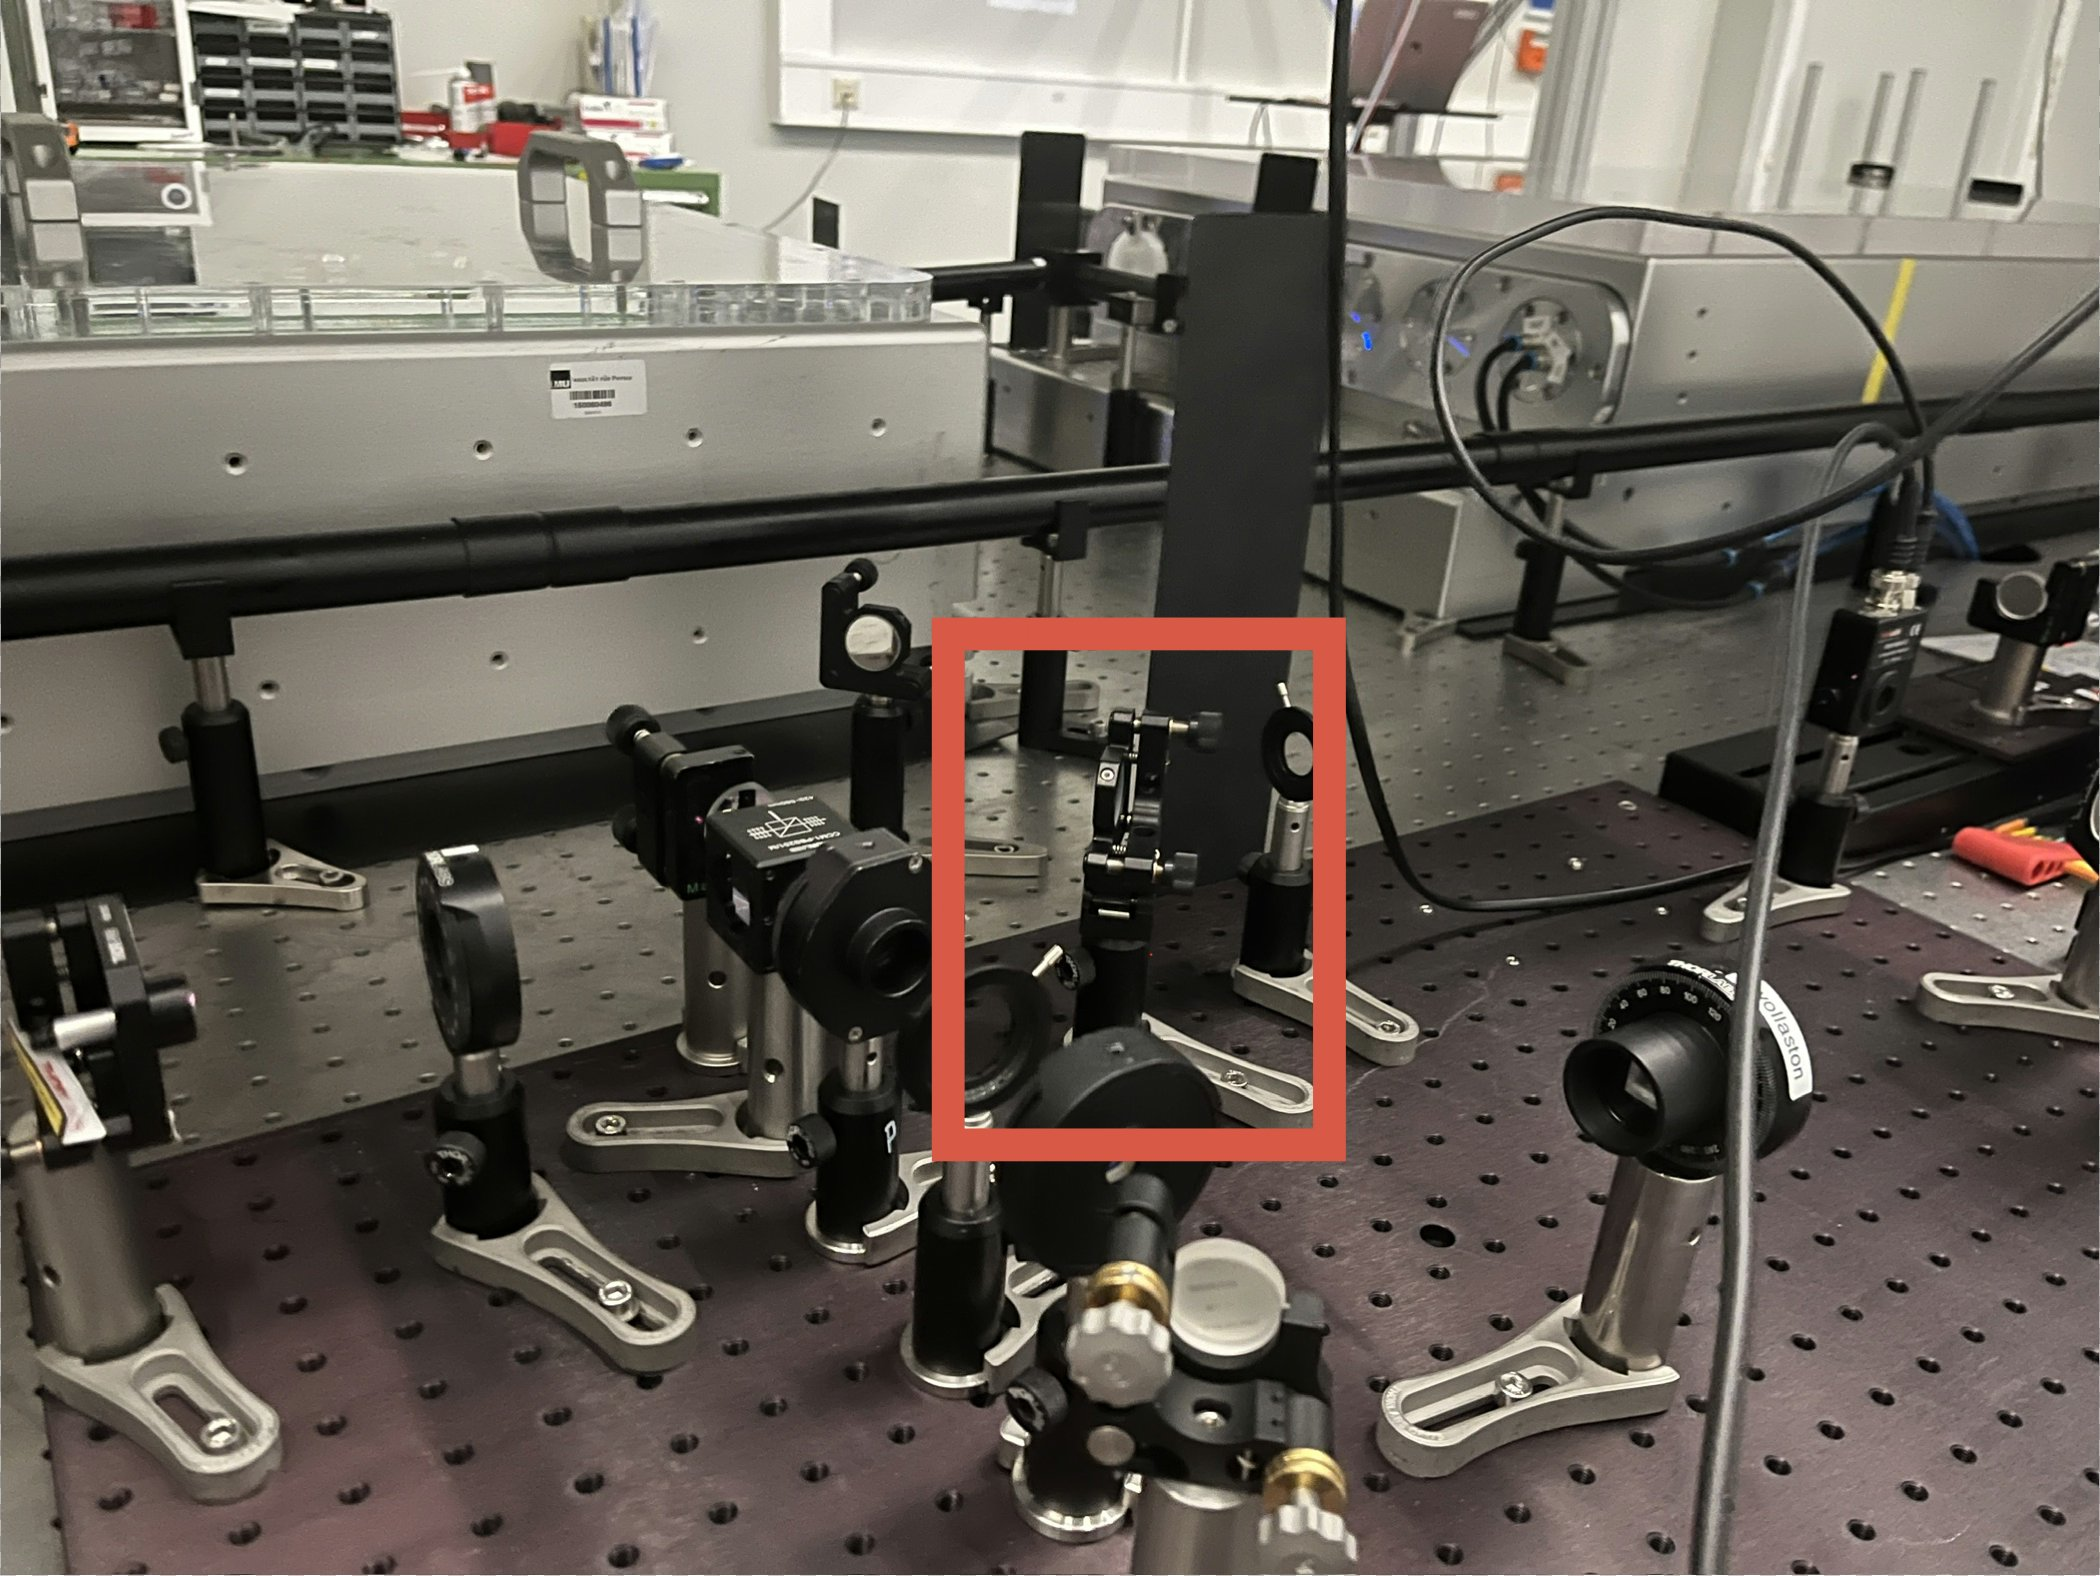
\includegraphics[width=\linewidth]{figures/withintegration.jpg}
    \end{minipage}\hfill
    \begin{minipage}{0.48\linewidth}
        \centering
        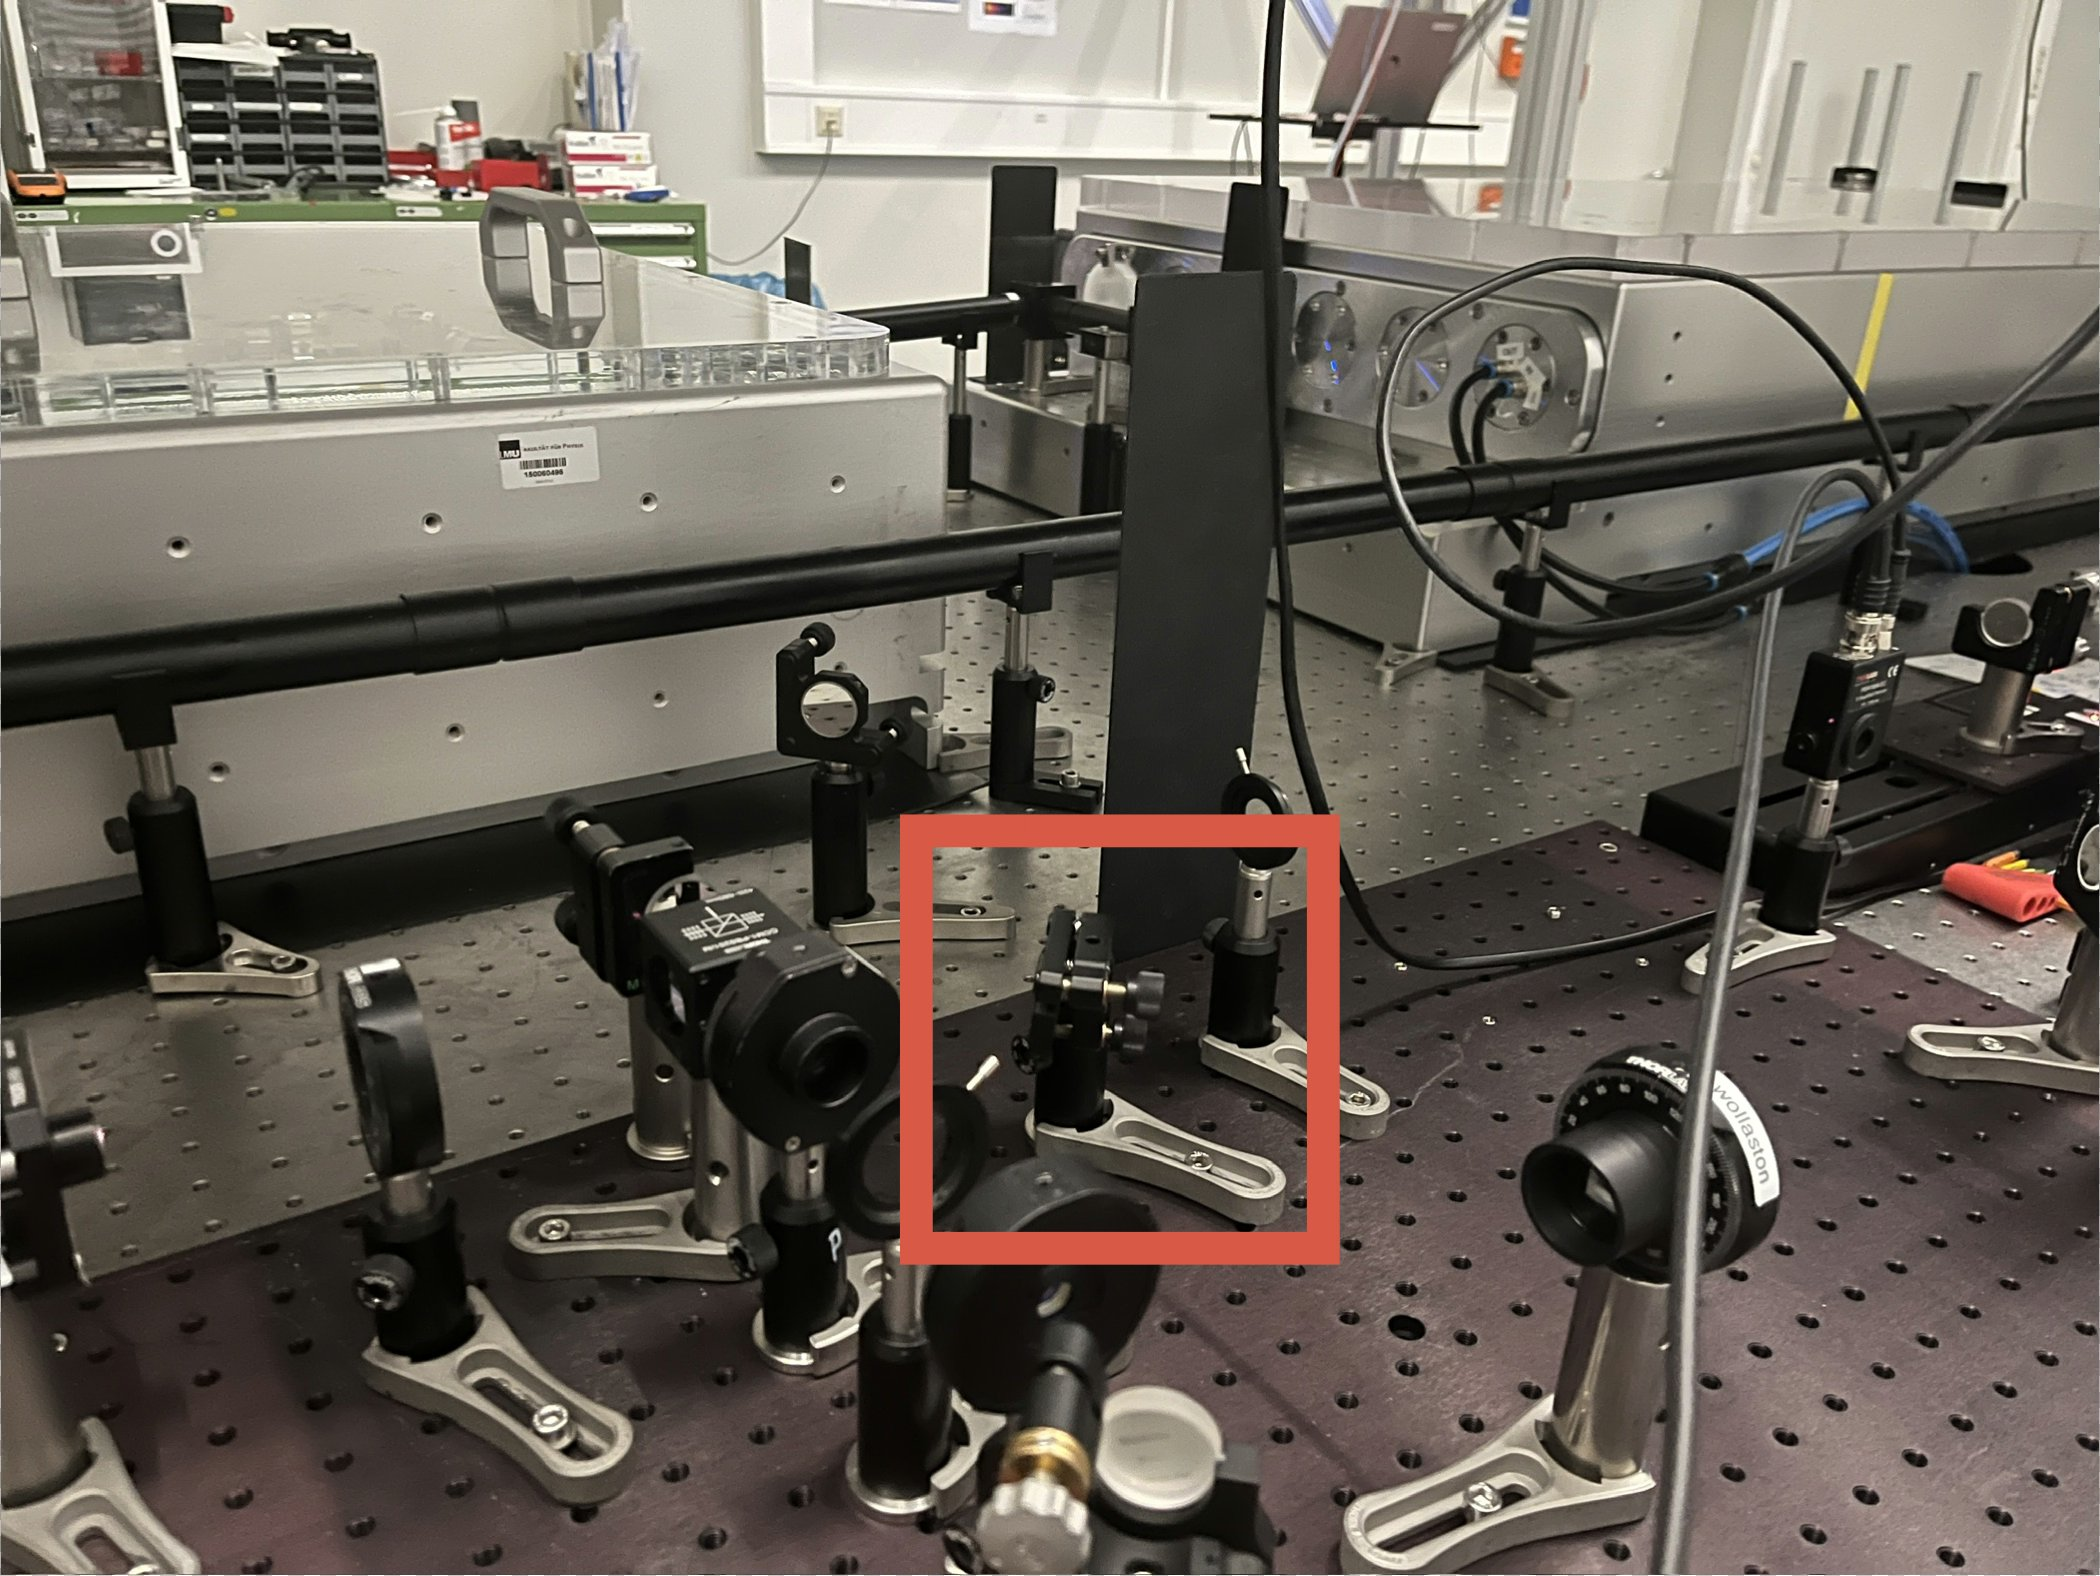
\includegraphics[width=\linewidth]{figures/withoutintegration.jpg}
    \end{minipage}
    \caption{Integration of the interferometer into the electro-optic sampling setup. Left: integrated configuration with the flip mirror raised, so that the signal from the external setup is coupled into the interferometer. Right: standalone configuration with the flip mirror lowered, so that the interferometer can be used with the local translation stage.}
    \label{fig:integration_flip_mirror}
\end{figure}

Due to the limited timeframe of this thesis, the integrated configuration could not be experimentally tested. However, since the interferometric measurement principle and the optical detection path remain unchanged, the setup is expected to be suitable for displacement measurements after careful alignment and calibration.
